\thispagestyle{myheadings}
\chapter{評価実験}

 収集した心拍データの心拍数上昇箇所の抽出処理が適切なのか,また表示したエフェクトが視聴者にはどのように感じるのかを評価するため実験を行う.
まずエフェクト重畳前の映画を視聴してもらった.安静にした状態で腕にスマートウォッチを取り付け,
映画を見る1分前から心拍数の取得を始め映画が終わるまでを計測した.環境は自宅でも気軽に臨場感が味わえることが目的なので,
普段映画を自宅で視聴する時と同じ環境で視聴した.次にエフェクトを重畳した映画も視聴してもらい,視聴後のアンケートも行った.

\section{心拍データの心拍数上昇箇所の抽出処理について}
 本節では心拍データの心拍数上昇箇所の抽出処理が適切に処理できていたか評価し考察する.

\subsection{心拍数上昇箇所の抽出方法についての評価}
 データを処理する際の閾値や設定が正確に処理できていたか評価する.
実験として3本の映画に対し各3人のデータを収集した.映画は 007/ノー・タイム・トゥ・ダイ,キングコング/髑髏島の巨神,嘘喰いの3本にした.
収集した心拍データを図\ref{king,usogui,nolimit}に示す.映画は心拍数の変化が大きくなると仮定したアクション映画にした.収集した心拍データを
観察したところ007の1人目のように徐々に心拍数が低くなっていく人や,嘘喰いの3人目のように徐々に心拍数が上がっていく人がいた.
また,キングコングの1人目と2人目や,007の2人目と3人目のように同じタイミングで心拍数が上昇している人たちもおり,心拍数が上昇した箇所は映画の盛り上がる
部分と一致していた.
\begin{figure}[H]
    \centering
    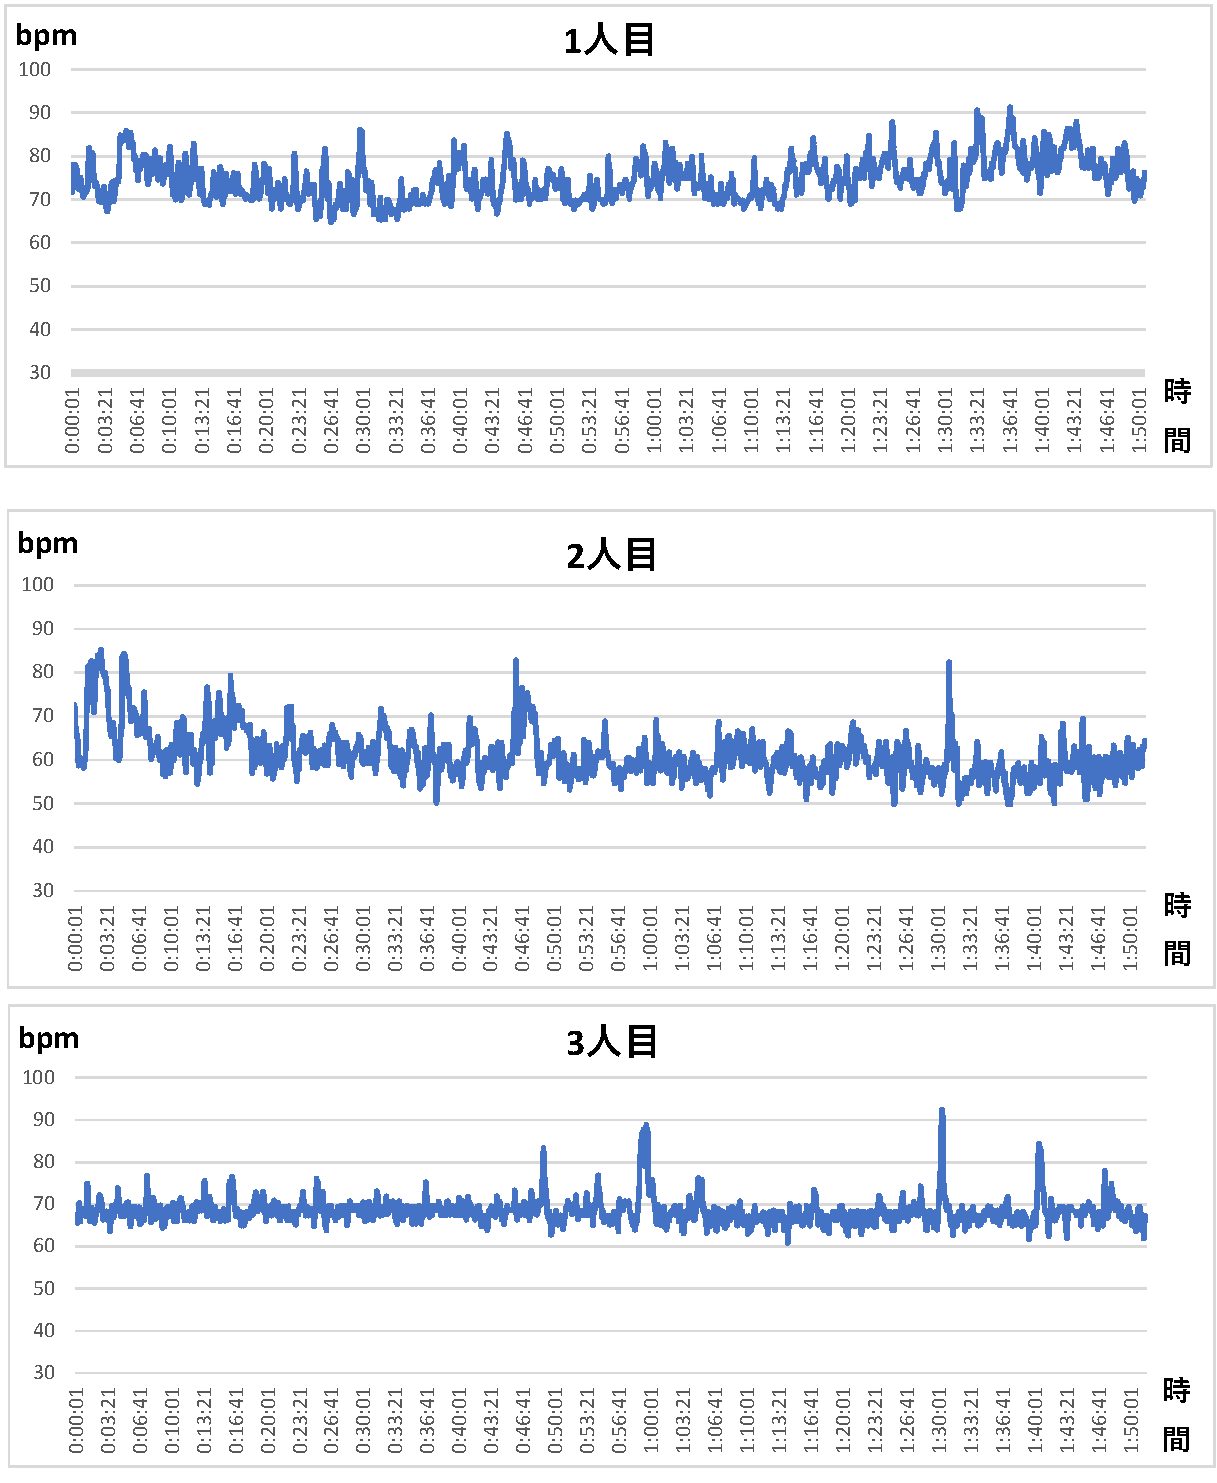
\includegraphics[width=14cm]{images/chapter4/kingkong2.pdf}
    \caption{キングコング 髑髏島の巨神を視聴した3人の心拍データ}
    \label{king}
\end{figure}
\begin{figure}[H]
    \centering
    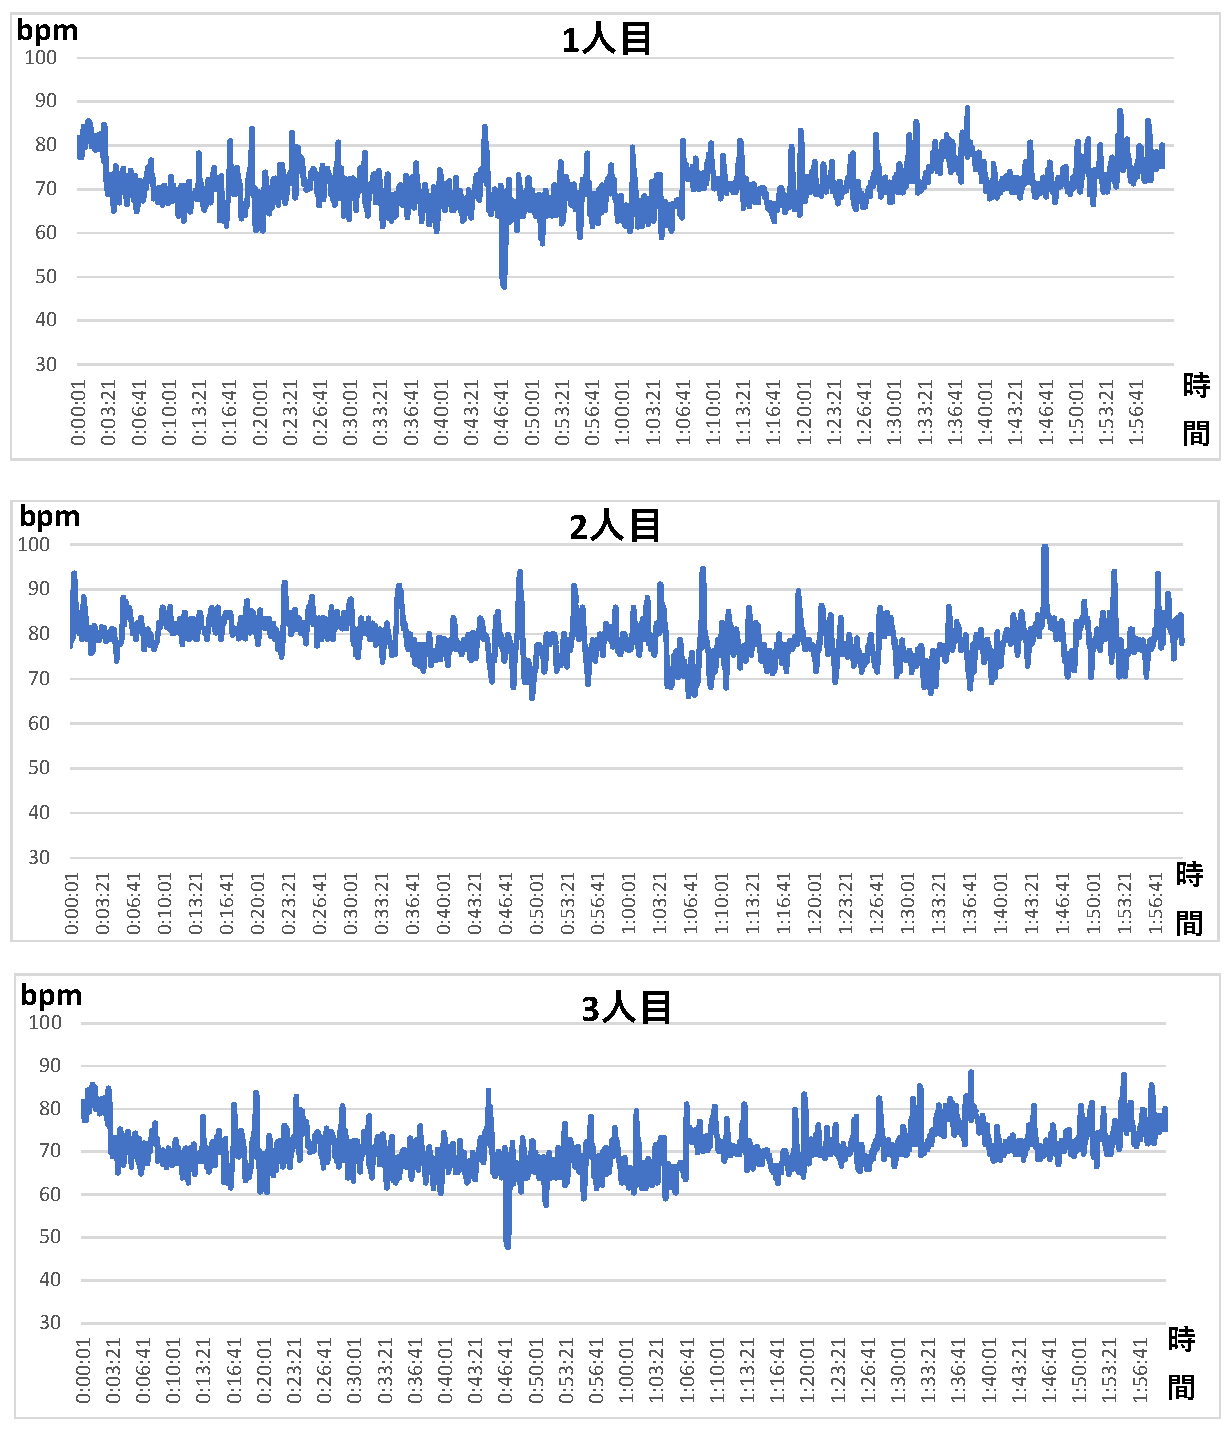
\includegraphics[width=14cm]{images/chapter4/usogui.pdf}
    \caption{嘘喰いを視聴した3人の心拍データ}
    \label{usogui}
\end{figure}
\begin{figure}[H]
    \centering
    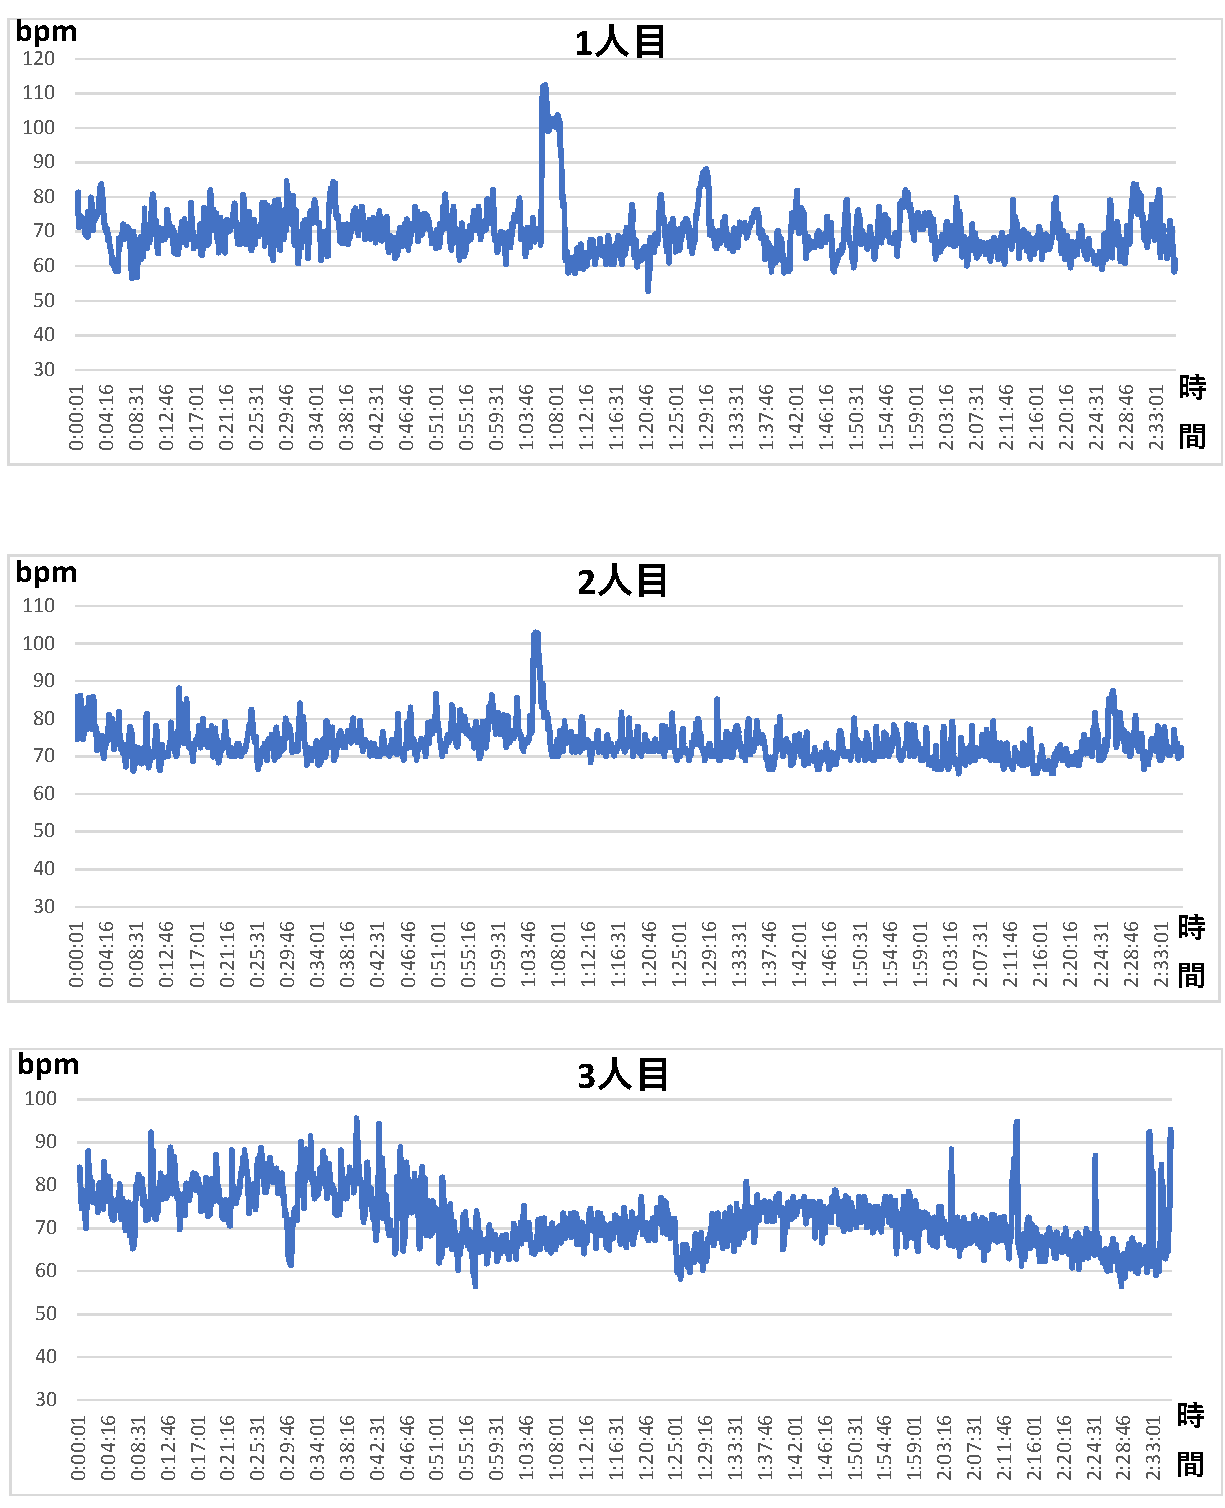
\includegraphics[width=14cm]{images/chapter4/nolimitto.pdf}
    \caption{007 nolimit to dieを視聴した3人の心拍データ}
    \label{nolimit}
\end{figure}

集めたデータを処理した結果について,盛り上がりのシーンで心拍数が上昇している部分が抜き出せているものもあった.
また,エフェクトを表示する時間fromからtoも閾値を超えた瞬間から下がるまでを記録できていた.
しかし人によっては心拍数が常に一定の人や変化が 激しい人などさまざまなためその全てに対応ができていなかった.
人によっては上昇箇所がたくさんあり,盛り上がりのシーン以外でも反応してしまった図\ref{kekka}.
また心拍数の変化が少ない人では全く心拍数の上昇箇所を抜き出すことができなかった.心拍数が上昇している箇所をうまく抜き出せていない映画では,
抽出処理した心拍データを1つのJSONデータにまとめる際に混ざってしまいうまく抜き出せている心拍データだけを反映するのができていなかった.


\begin{figure}[H]
    \centering
    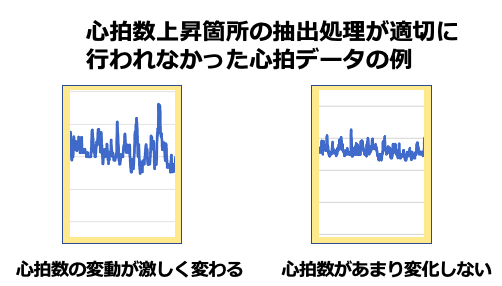
\includegraphics[width=10cm]{images/chapter4/miss.png}
    \caption{適切に抽出処理ができていなかった例}
    \label{kekka}
\end{figure}


\subsection{心拍数上昇箇所の抽出方法についての考察}
 心拍数が上昇している箇所を適切に抜き出せていない原因として,
始めの一分間を安静時の心拍数として決定するためその後の変化に対応できないからだと推測する.
はじめの1分間を安静時の心拍数として決定すると,
映画が進むにつれ徐々に心拍数が上がっていく人や逆に下がっていく人など閾値の設定が反映されなくなってしまったからだと考える.
また図\ref{kekka2}のように映画を見る前の状態では落ち着いた心拍数で安定しているが,
映画を見始めると心拍数が安定していても興奮しているため平均心拍数が安静時よりも高くなっているからである.
 最終的に一つのJSONデータにまとめる際に盛り上がりのシーン以外も使いされてしまう課題について,
処理したそれぞれの心拍データを一つのJSONデータに追加していくだけなので,
姿勢を変えたなどのノイズもエフェクト表示に使われてしまった.対策として様々な心拍数の変化に対応するため,
平均を常に更新しそれに応じて閾値も変動させ,データを一つにまとめる際には複数人が反応を示している箇所だけを抜き出しまとめれば解決すると考える. 

\begin{figure}[H]
    \centering
    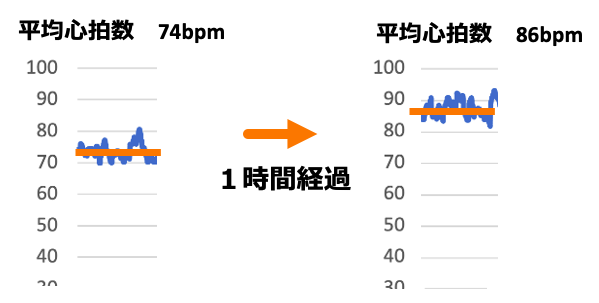
\includegraphics[width=13cm]{images/chapter4/bpmave.png}
    \caption{平均心拍数の推移}
    \label{kekka2}
\end{figure}

\section{エフェクト重畳提示について}
本節では,エフェクト重畳提示が適切に提示できていたか評価し考察する.
エフェクト選択後の視聴画面に対して10人分のアンケートデータを取集し,評価方法としてGoogleFormsを使用し,エフェクト制作の目的を1から5段階評価でどれほどエフェクトの目的を感じたかを収集した.

\subsection{エフェクト重畳提示についての評価}

 エフェクト重畳された動画と何も重畳していない動画を視聴し,適切に提示できていたかを評価する.評価する項目として,性別,年齢,エフェクトの評価,エフェクトの意見/感想の4項目である.
Actionのエフェクトでは「キングコング/ 髑髏島の巨神」を視聴し5の評価を4件,4の評価を6件の結果が得られた.意見/感想では,緊迫感が表されていて良いと思った,赤色のエフェクトのみなのか,もう少しエフェクトを細くしてもいいかも,映像が見づらくなる時がある,動きが重なってしまう,急に消えてしまう,心拍が高くなっているのが分かりやすいがあげられた.Animeのエフェクトでは「SPY×FAMILY/エピソード6」を視聴し5の評価を3件,4の評価を7件の結果が得られた.意見/感想では,効果線として合うシーンに使えれば良い印象,効果線をかぶせるのは面白いと感じた,効果線の主張を少し弱くする,線が多すぎる,主張を弱くする,白と黒の線が気になる,ジャンルがあっていれば面白くなるかもがあげられた.Horrorのエフェクトでは「嘘喰い」を視聴し4の評価を4件,3の評価を6件の結果が得られた.意見/感想では,見えなくなった,見やすくなっていた,もう少し見やすくしてほしい,映像の邪魔になっている,黒の方がいい,逆に怖くしたいがあげられた.その他意見/感想で,映画やアニメは完成されたものが上映されているので,あまり主張が強すぎると逆に違和感が出てくるかもしれないと思った.映像では意見が難しい点や実際に体験したら意見が変化すると感じる点があげられる.

\subsection{エフェクト重畳提示についての考察}
Actionの評価の原因として,意見/感想の赤色のエフェクトのみなのは赤色のみの表示になっているためアクション映画の中でも赤色のエフェクト以外を選択できるようにエフェクト選択する際に,色設定の項目を追加する.もう少しエフェクトを細くする/見づらくなる時があるでは,AftetEffectsで両脇の横サイズをせばめる.動きが重くなってしまう/急に消えてしまうは,AftetEffectsでモーションブラーを追加しフェードアウトを追加することで解決すると考える.
Animeの評価の原因として,意見/感想の効果線として合うシーンに使えれば良い印象/ジャンルがあっていれば面白くなるかもはアニメの中でもコメディやSFなど多くのジャンルがあるため,アニメのエフェクトの種類を増やす.効果線の主張を少し弱くする/線が多すぎるは,Illastratorで線の幅と本数を減らす,白と黒の線が気になるは,効果線の効果として必要であるためエフェクトのジャンルと種類を増やすことで解決すると考える.
Horrorの評価の原因として,意見/感想の見えなくなった/もう少し見やすくしてほしい/映像の邪魔になっているは,AftetEffectsで全体にフラクタルノイズをかけているが,四隅に設置することで映像視聴に影響が出ないようにする.黒の方がいいは,ホラーの中でも明るい動画のときに使用できるように色の種類を選択可能にする.逆に怖くしたいは,ホラーの目的とは別になるがさらに恐怖感を体験できる目的として制作することで解決できると考える.
